\documentclass[10pt]{beamer}

\usetheme[progressbar=frametitle]{metropolis}
\usepackage{appendixnumberbeamer}

\usepackage{booktabs}
\usepackage[scale=2]{ccicons}

\usepackage{pgfplots}
\usepgfplotslibrary{dateplot}

\usepackage{xspace}
\newcommand{\themename}{\textbf{\textsc{metropolis}}\xspace}

\usepackage{bm}

\title{Genetic load and efficacy of selection on admixed populations}
\subtitle{A Diffusion Processes Approach}
% \date{\today}
\date{}
\author{Jonatas Cesar}
\institute{University of S\~ao Paulo \& University of Chicago}
% \titlegraphic{\hfill\includegraphics[height=1.5cm]{logo.pdf}}

\begin{document}

\maketitle

\begin{frame}{Table of contents}
  \setbeamertemplate{section in toc}[sections numbered]
  \tableofcontents[hideallsubsections]
\end{frame}

\section{Quick Bio}

\begin{frame}{Statistical Mechanics of Interacting Bayesian Agents: Applications
    to Moral Foundation Theory}
  \begin{itemize}
      \item $\bm \omega_i$: agent moral vector 
      \item $\bm x$: random issues 
      \item $\mathcal H$: Cost of disagreement between agents
  \end{itemize}
  
  Socio-dynamic sketch:
  \[
    \bm \omega_i^{t + 1} = \bm \omega_i^{t} + 
    \eta \bm \nabla 
    \mathcal H (\bm \omega_i^t \cdot \bm x ^t, \bm \omega_j^t \cdot \bm x ^t)
  \]

  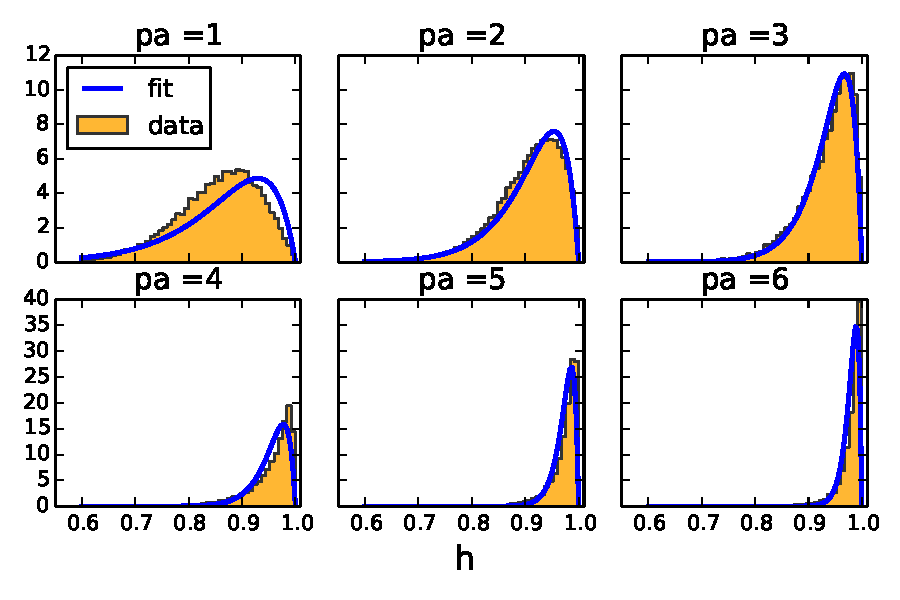
\includegraphics[width=0.45\textwidth]{./Figures/mf_usa}
  \hspace{5pt}
  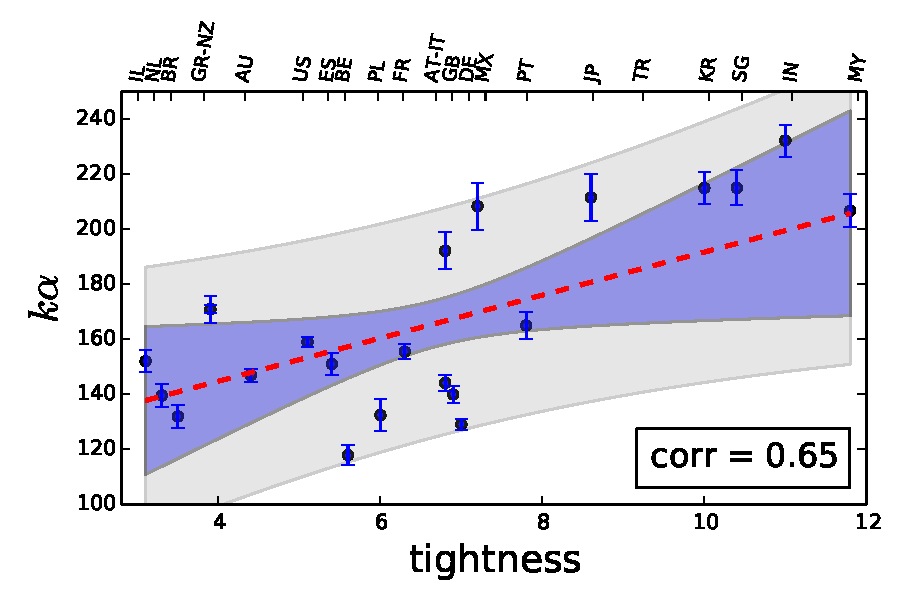
\includegraphics[width=0.45\textwidth]{./Figures/beta_tight.pdf}
  \let\thefootnote\relax\footnote{J. Cesar and N. Caticha, in prep}
\end{frame}

\begin{frame}{SUVREL: Supervised Variational Relevance Learning}

  \begin{alertblock}{Objective}
  Learning a metric tensor $g_{\mu\nu}$ on the feature space that minimizes
  intra-groups distances and maximize inter-groups distances. 
	\end{alertblock}
  \[
    E = \sum_{intra(i,j)} d_{ij} - \gamma \sum_{iter(i,j)} d_{ij}, 
  \]
  $d_{ij}$ are defined as a quadratic distance in the new space $X' = G X$ 

  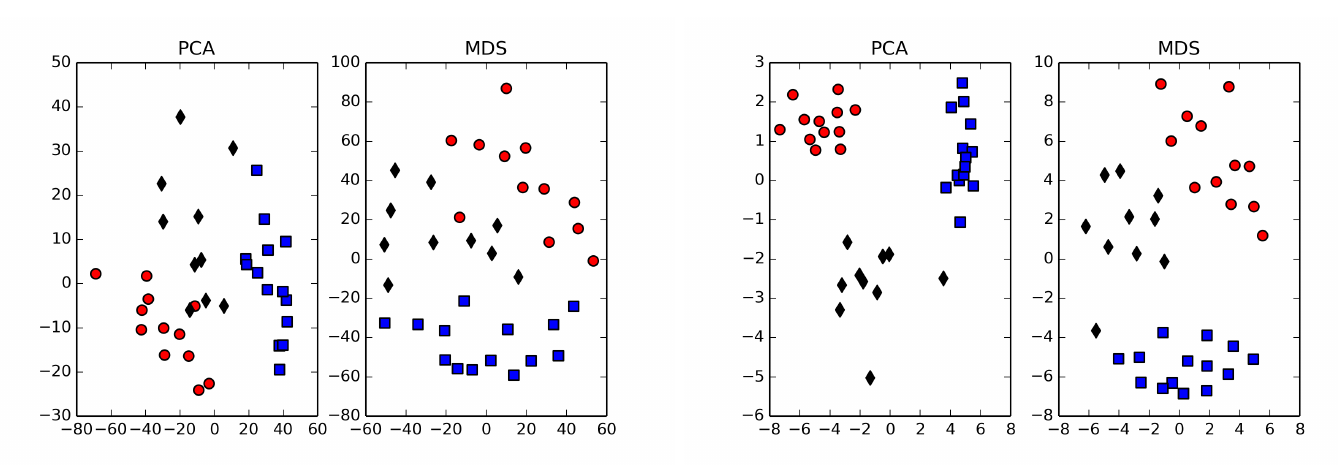
\includegraphics[width=\textwidth]{./Figures/suvrel_image.png}
  \let\thefootnote\relax\footnote{M. Boareto, J. Cesar, V.B. Leite and
    N. Caticha. IEEE/ACM Transactions in Computational Biology and
    Bioinformatics (2015)}
\end{frame}

\section{Recent Projects on Popgen}

\begin{frame}{Expression estimation and eQTL mapping of HLA genes}
  \centering
  \begin{minipage}{0.6\textwidth}
  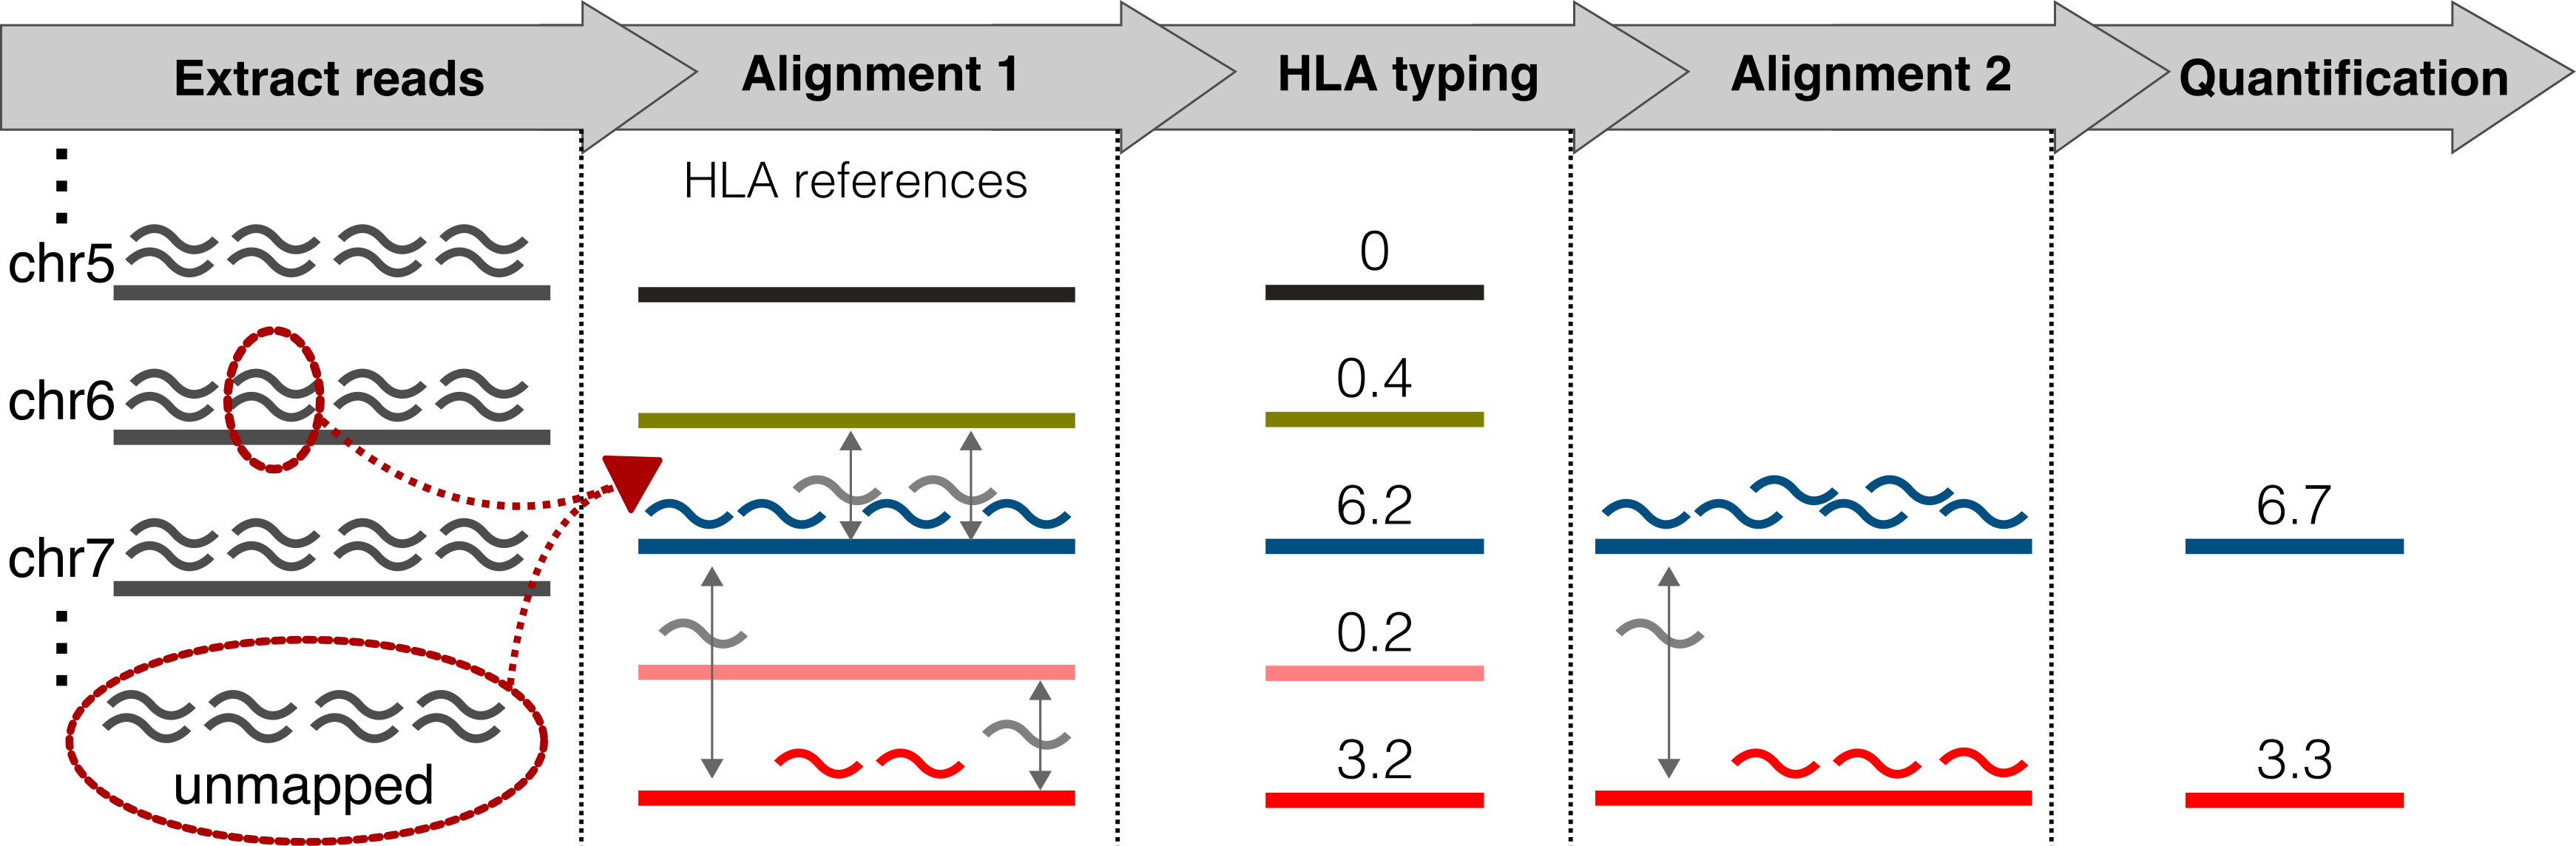
\includegraphics[width=\textwidth]{./Figures/method.png}
  \end{minipage}
  \hspace{5pt}
  \begin{tiny}
  \begin{tabular}{lc}
    \hline
    Gene & accuracy (\%) \\
    \hline
    A & 98.5  \\
    B & 98.5  \\
    C & 97.5  \\
    DQB1 & 98.5  \\
    DRB1 & 99.5  \\
    \hline
  \end{tabular}
  \end{tiny}
  \vfill

  \begin{minipage}{0.5\textwidth}
  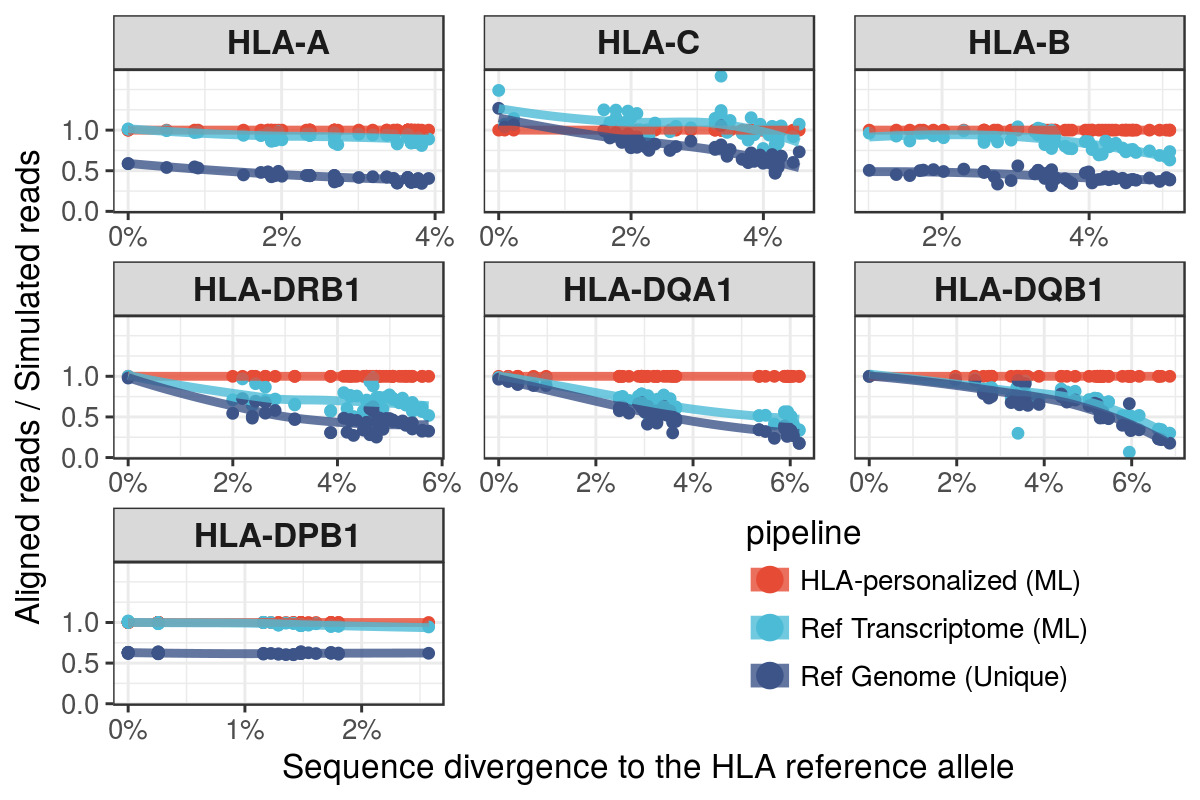
\includegraphics[width=\textwidth]{./Figures/prop_mapped_divergence.png}
  \end{minipage}
  \begin{minipage}{0.45\textwidth}
  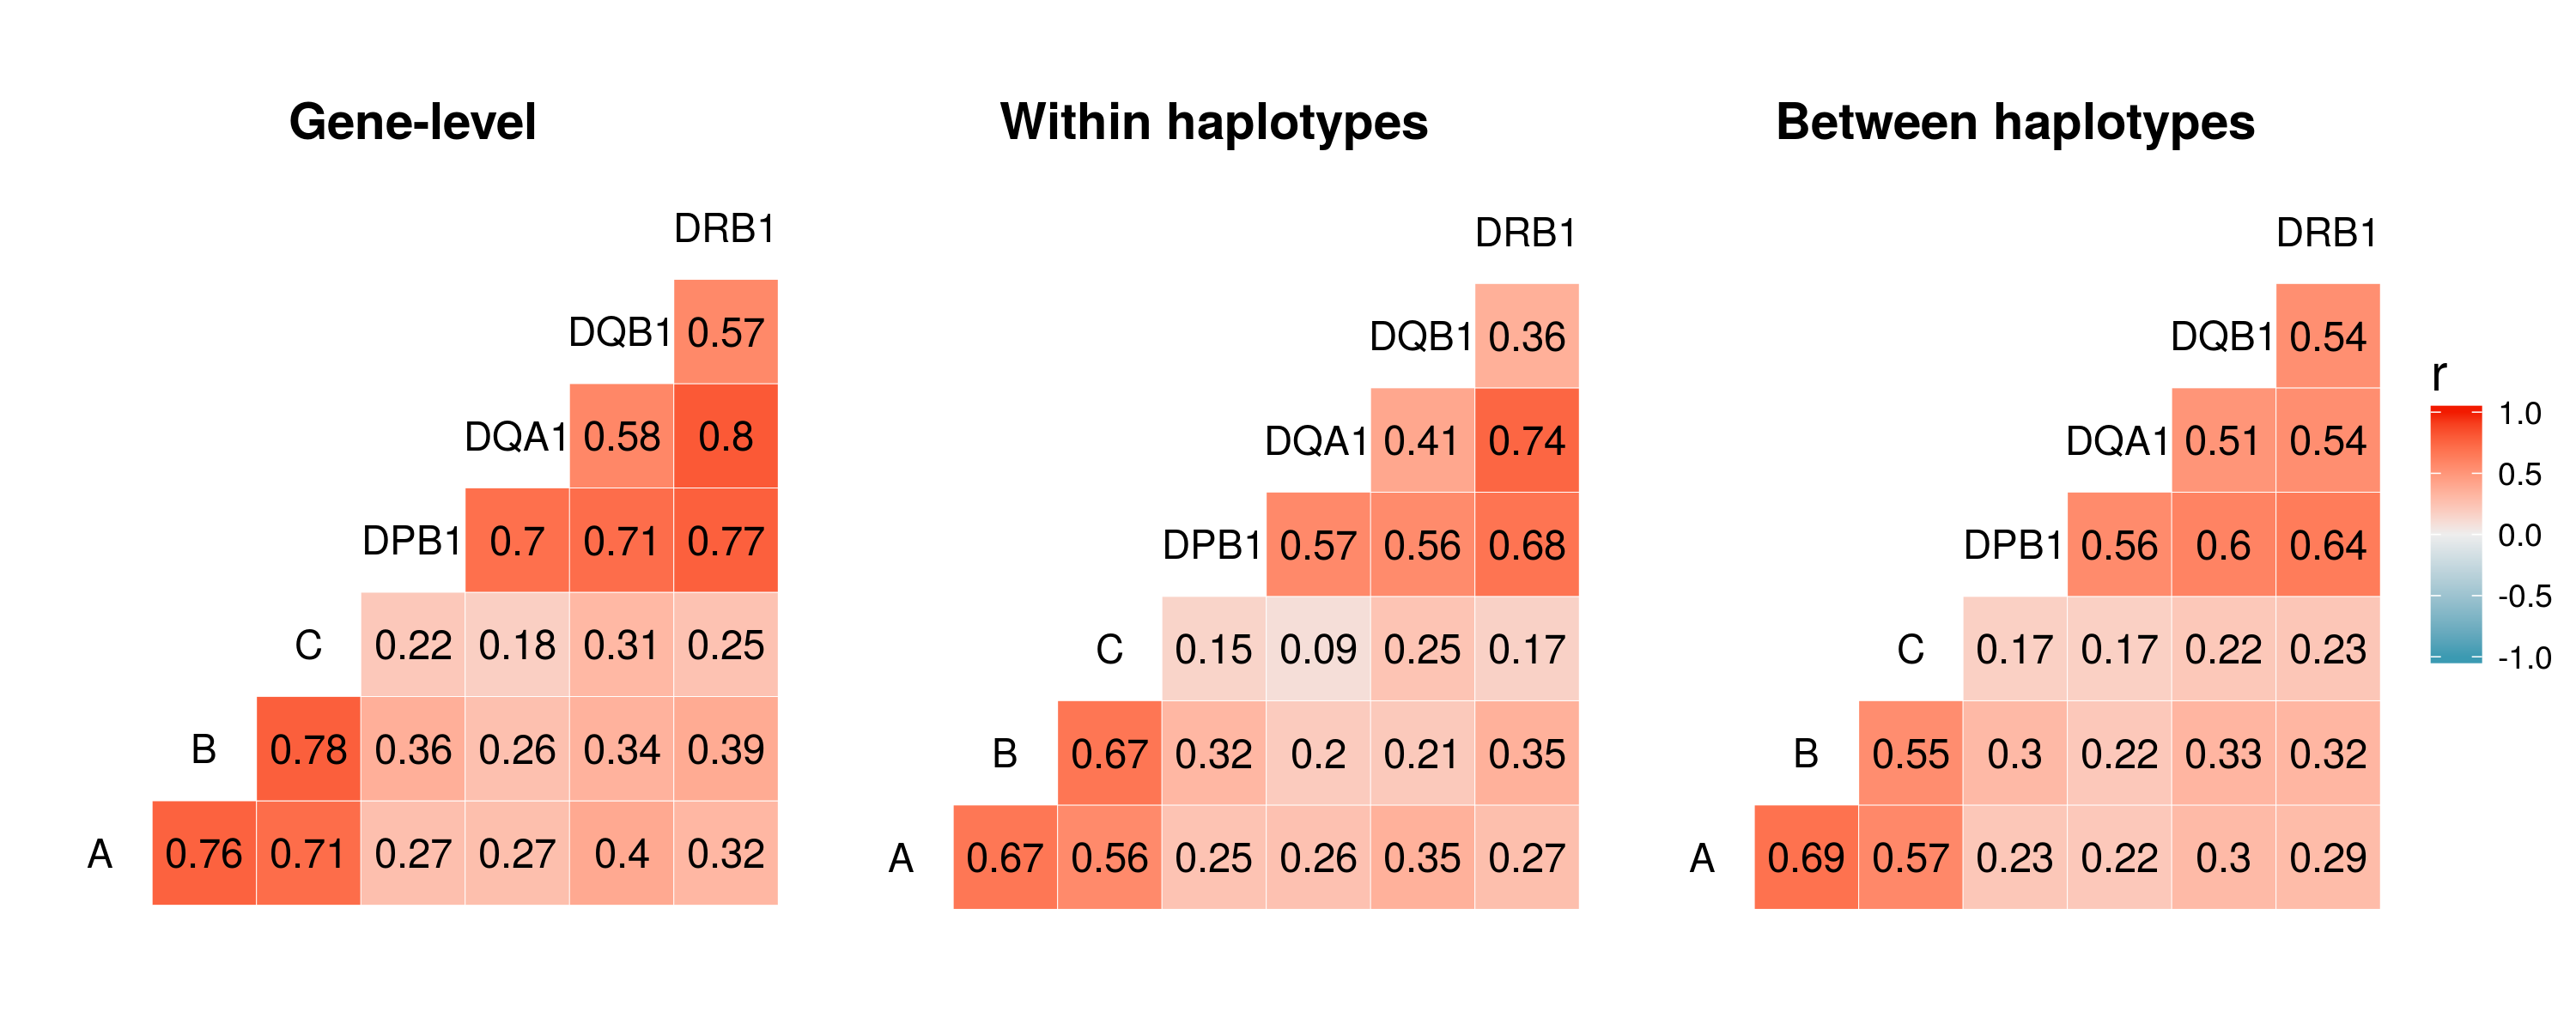
\includegraphics[width=\textwidth]{./Figures/correlations.png}
  \end{minipage}

\end{frame}

\begin{frame}{\small The effect of balancing selection on population
    differentiation:\\ a study with HLA genes}
  \centering
  \begin{minipage}{0.43\textwidth}
    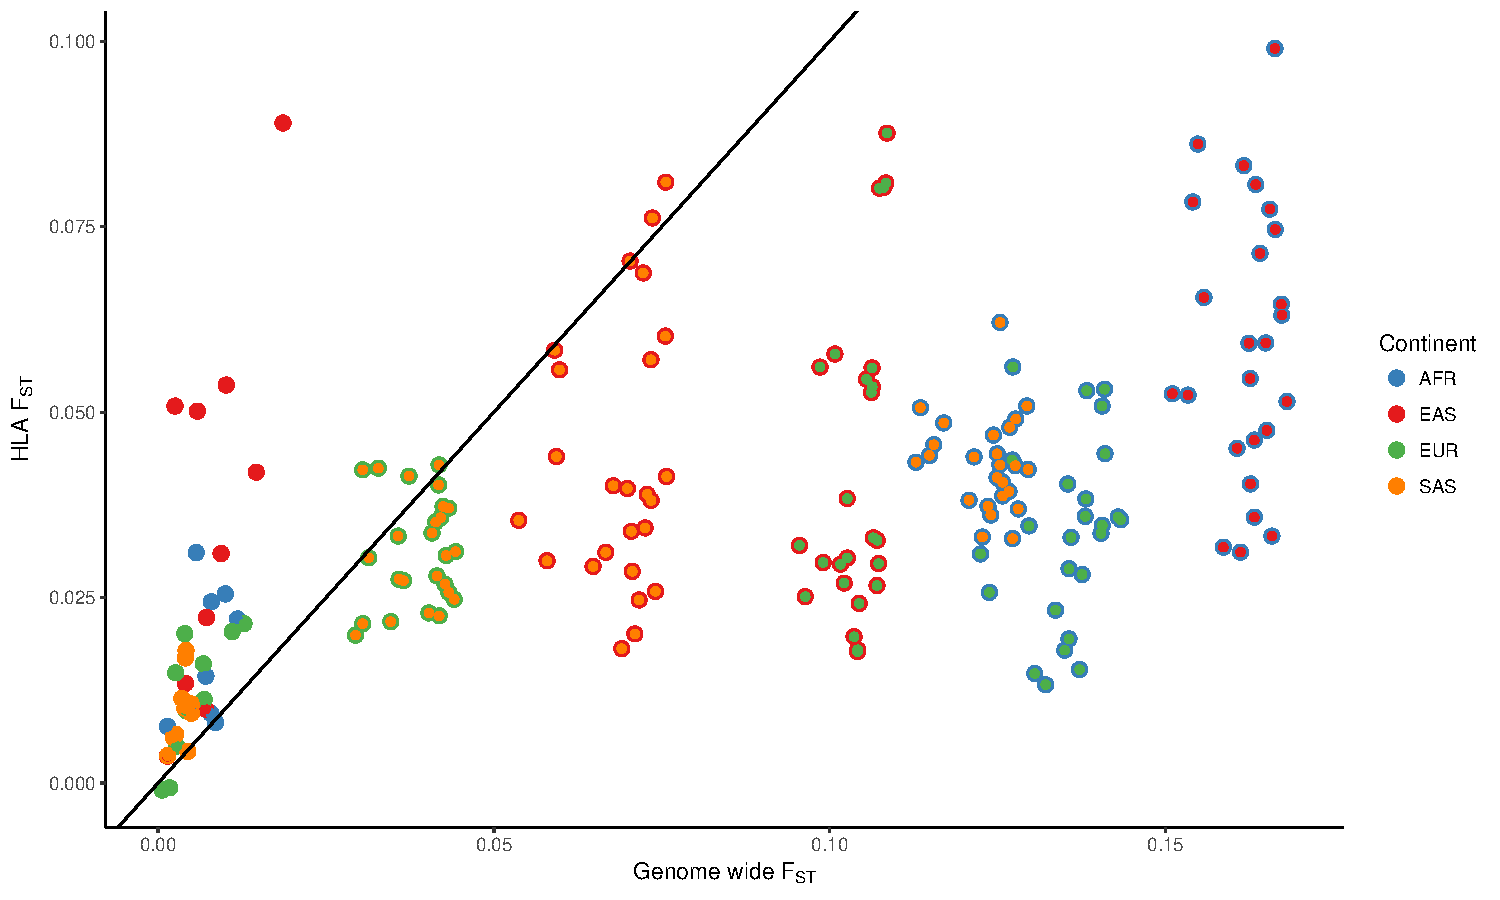
\includegraphics[width=\textwidth]{./Figures/pw_fst.pdf}
  \end{minipage}
  \begin{minipage}{0.43\textwidth}
    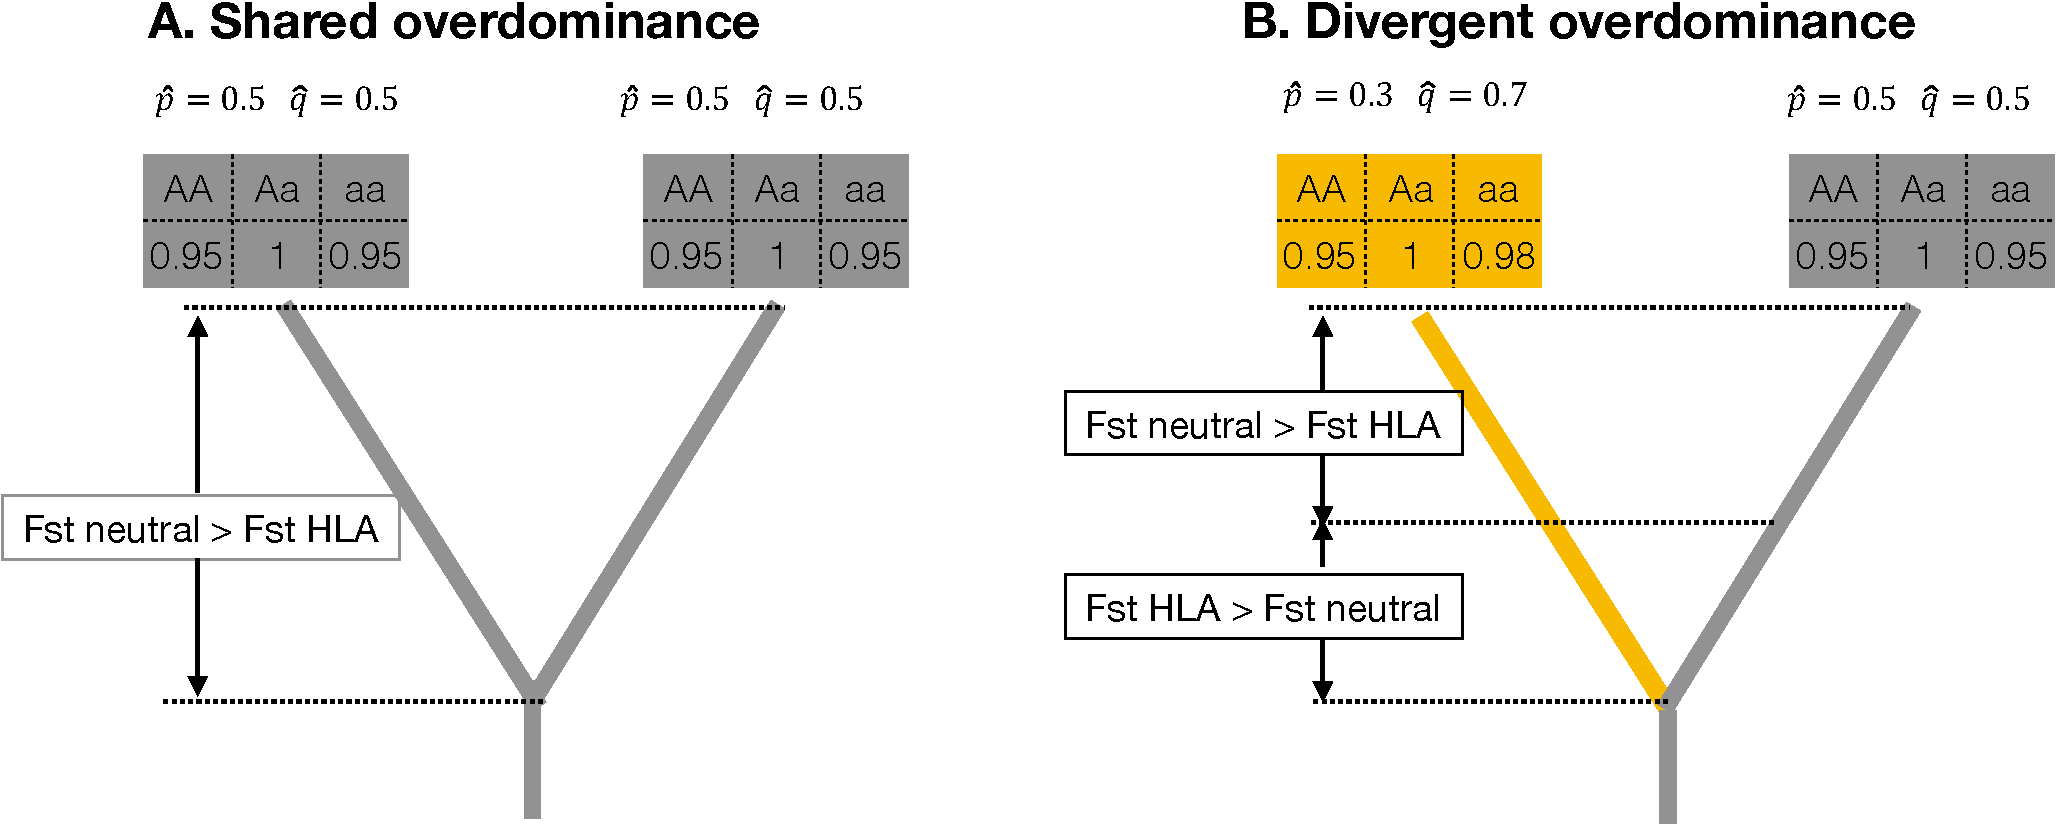
\includegraphics[width=\textwidth]{./Figures/fig_od.pdf}
  \end{minipage}
  \begin{minipage}{0.43\textwidth}
    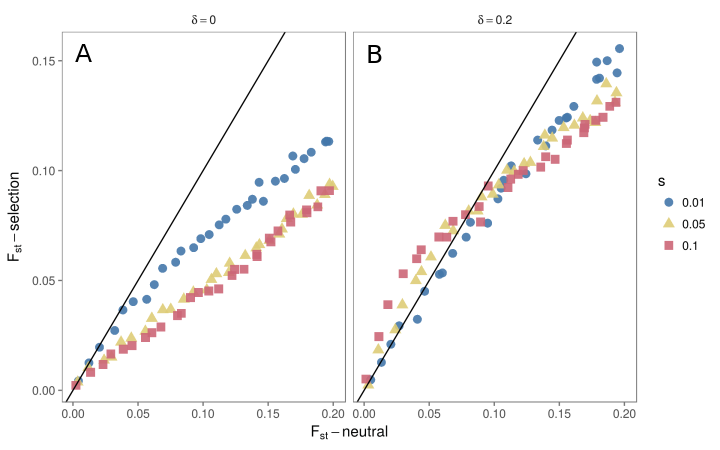
\includegraphics[width=\textwidth]{./Figures/bsel_x_neu_simple_1.png}
  \end{minipage}
  \begin{minipage}{0.43\textwidth}
    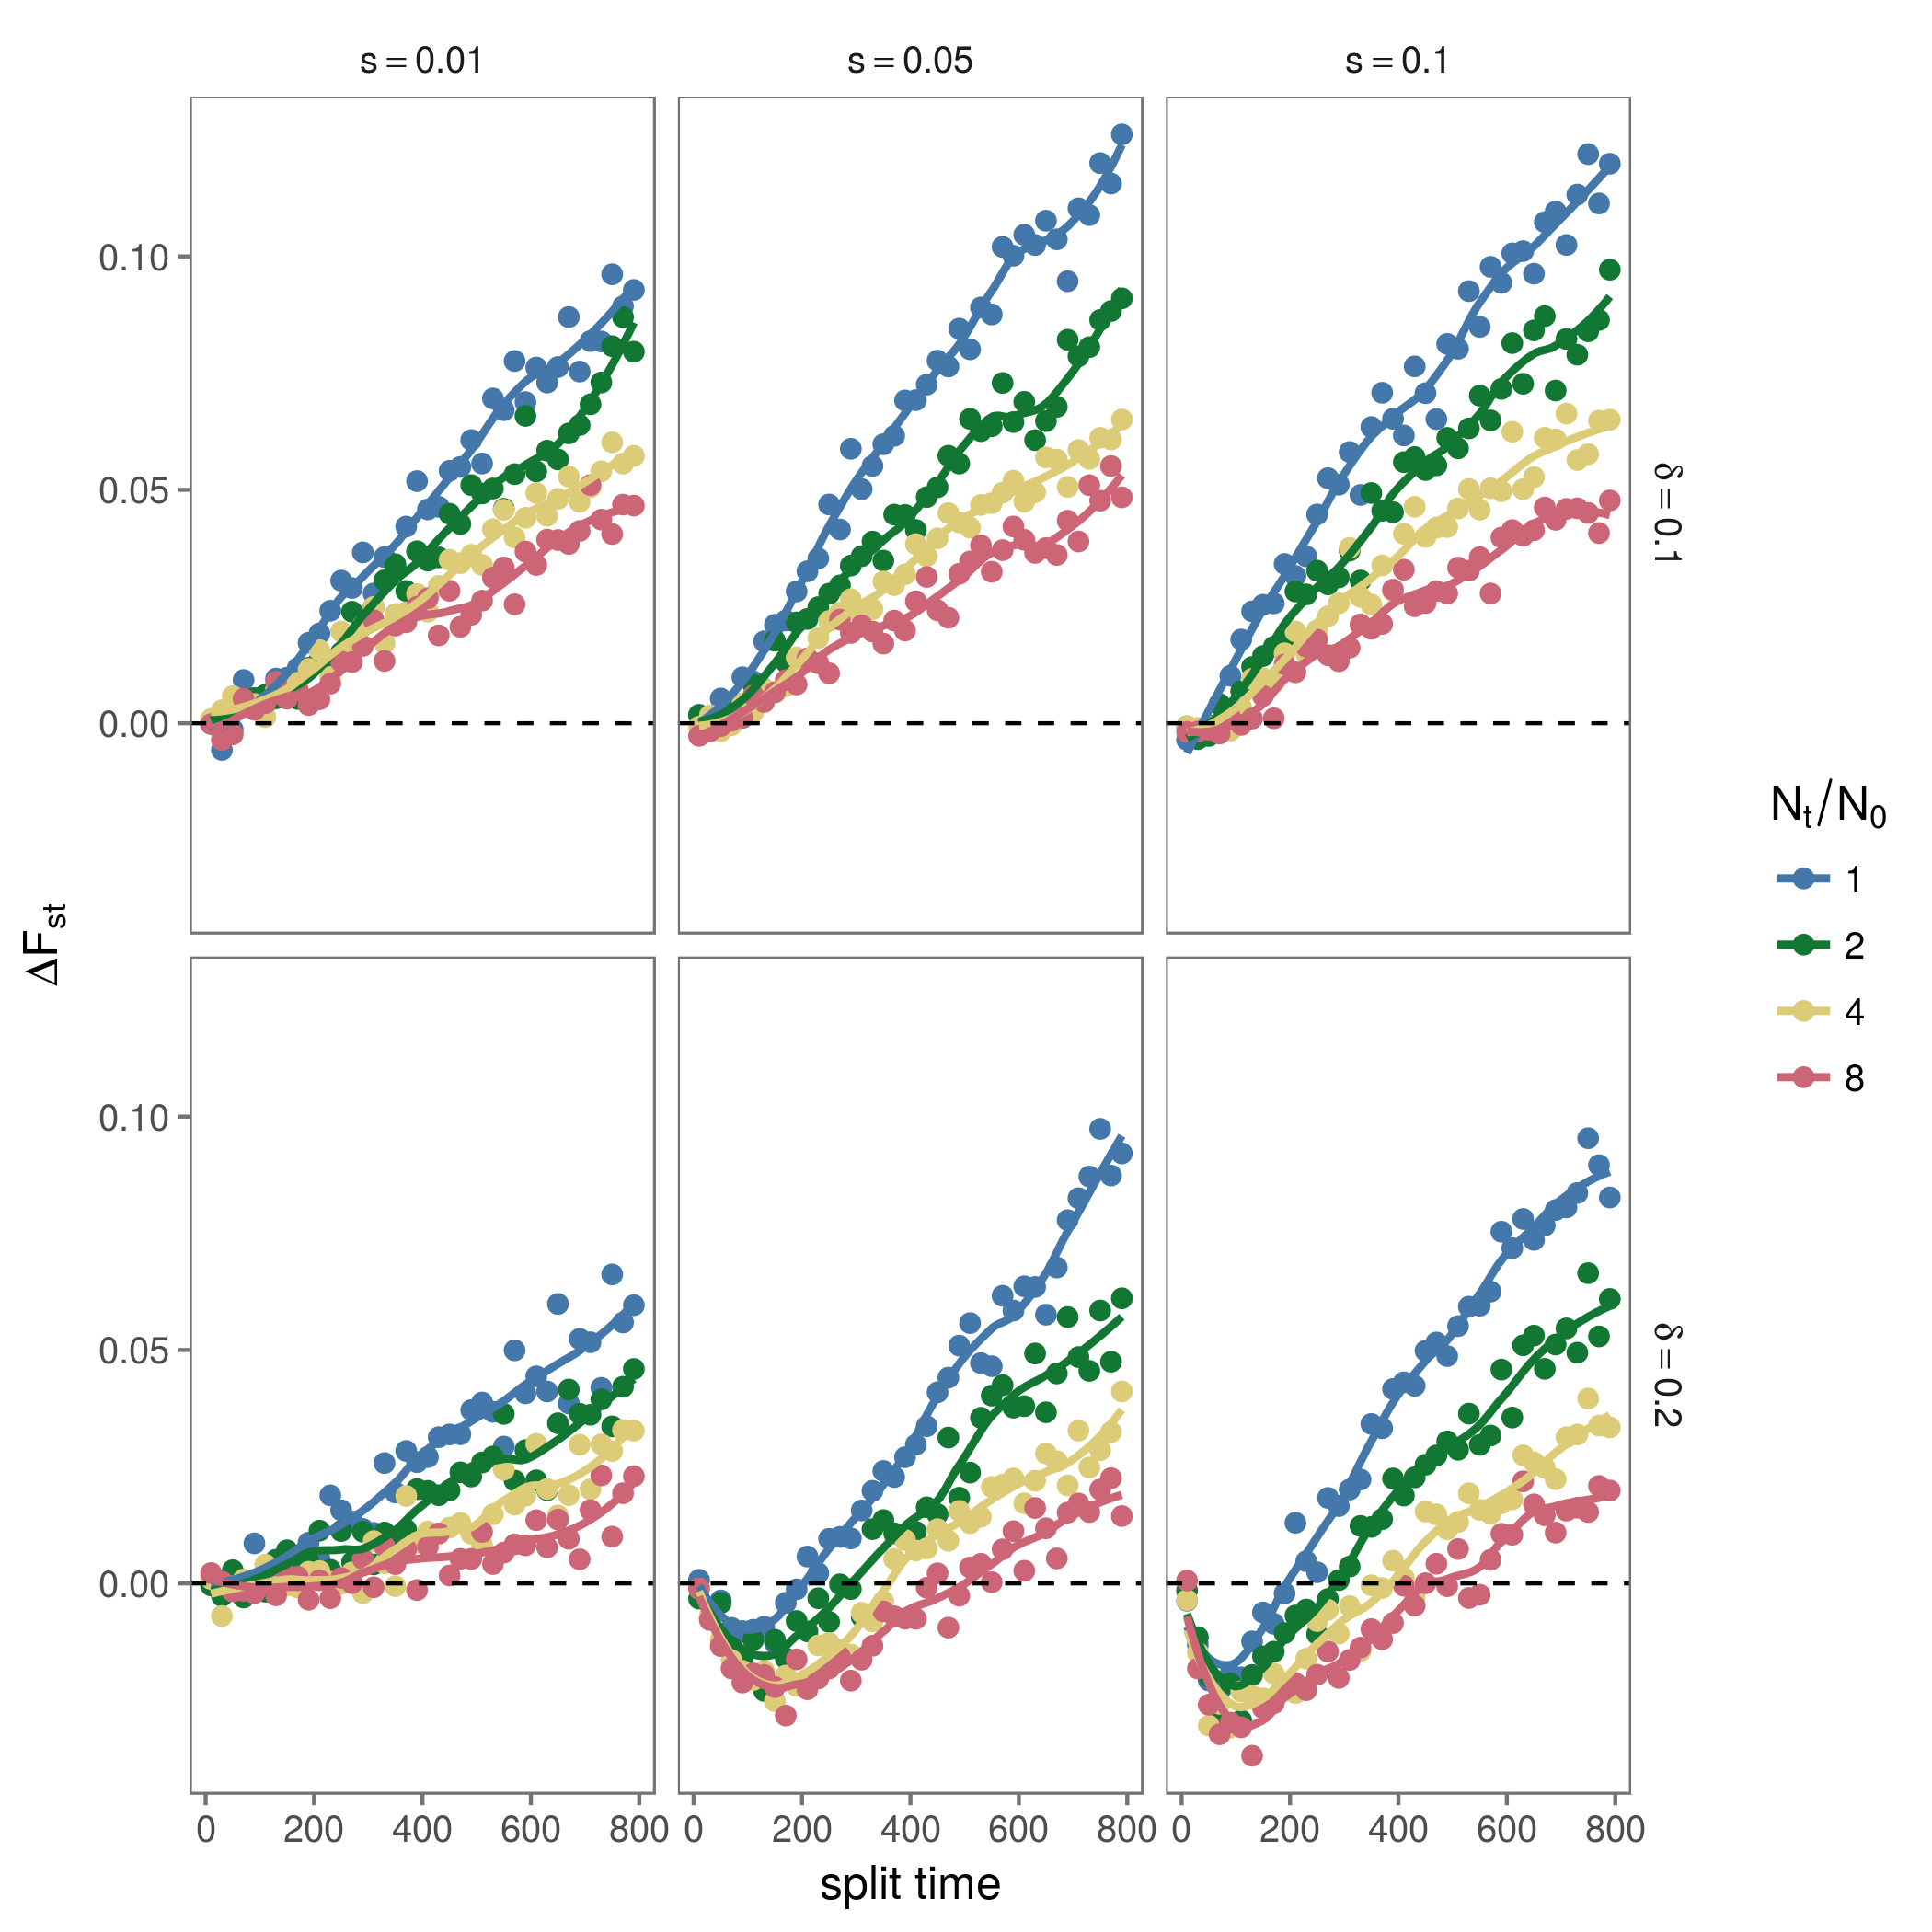
\includegraphics[width=\textwidth]{./Figures/DFst_zoom.png}
  \end{minipage}
  \let\thefootnote\relax\footnote{D. Brandt, J. Cesar, J. Goudet, D. Meyer G3
    (2018)}
\end{frame}

\begin{frame}{\small The cost of selection: how balancing selection at HLA
    impacts  \\ their genomic neighbourhood}
  \centering
  \begin{minipage}{0.35\textwidth}
    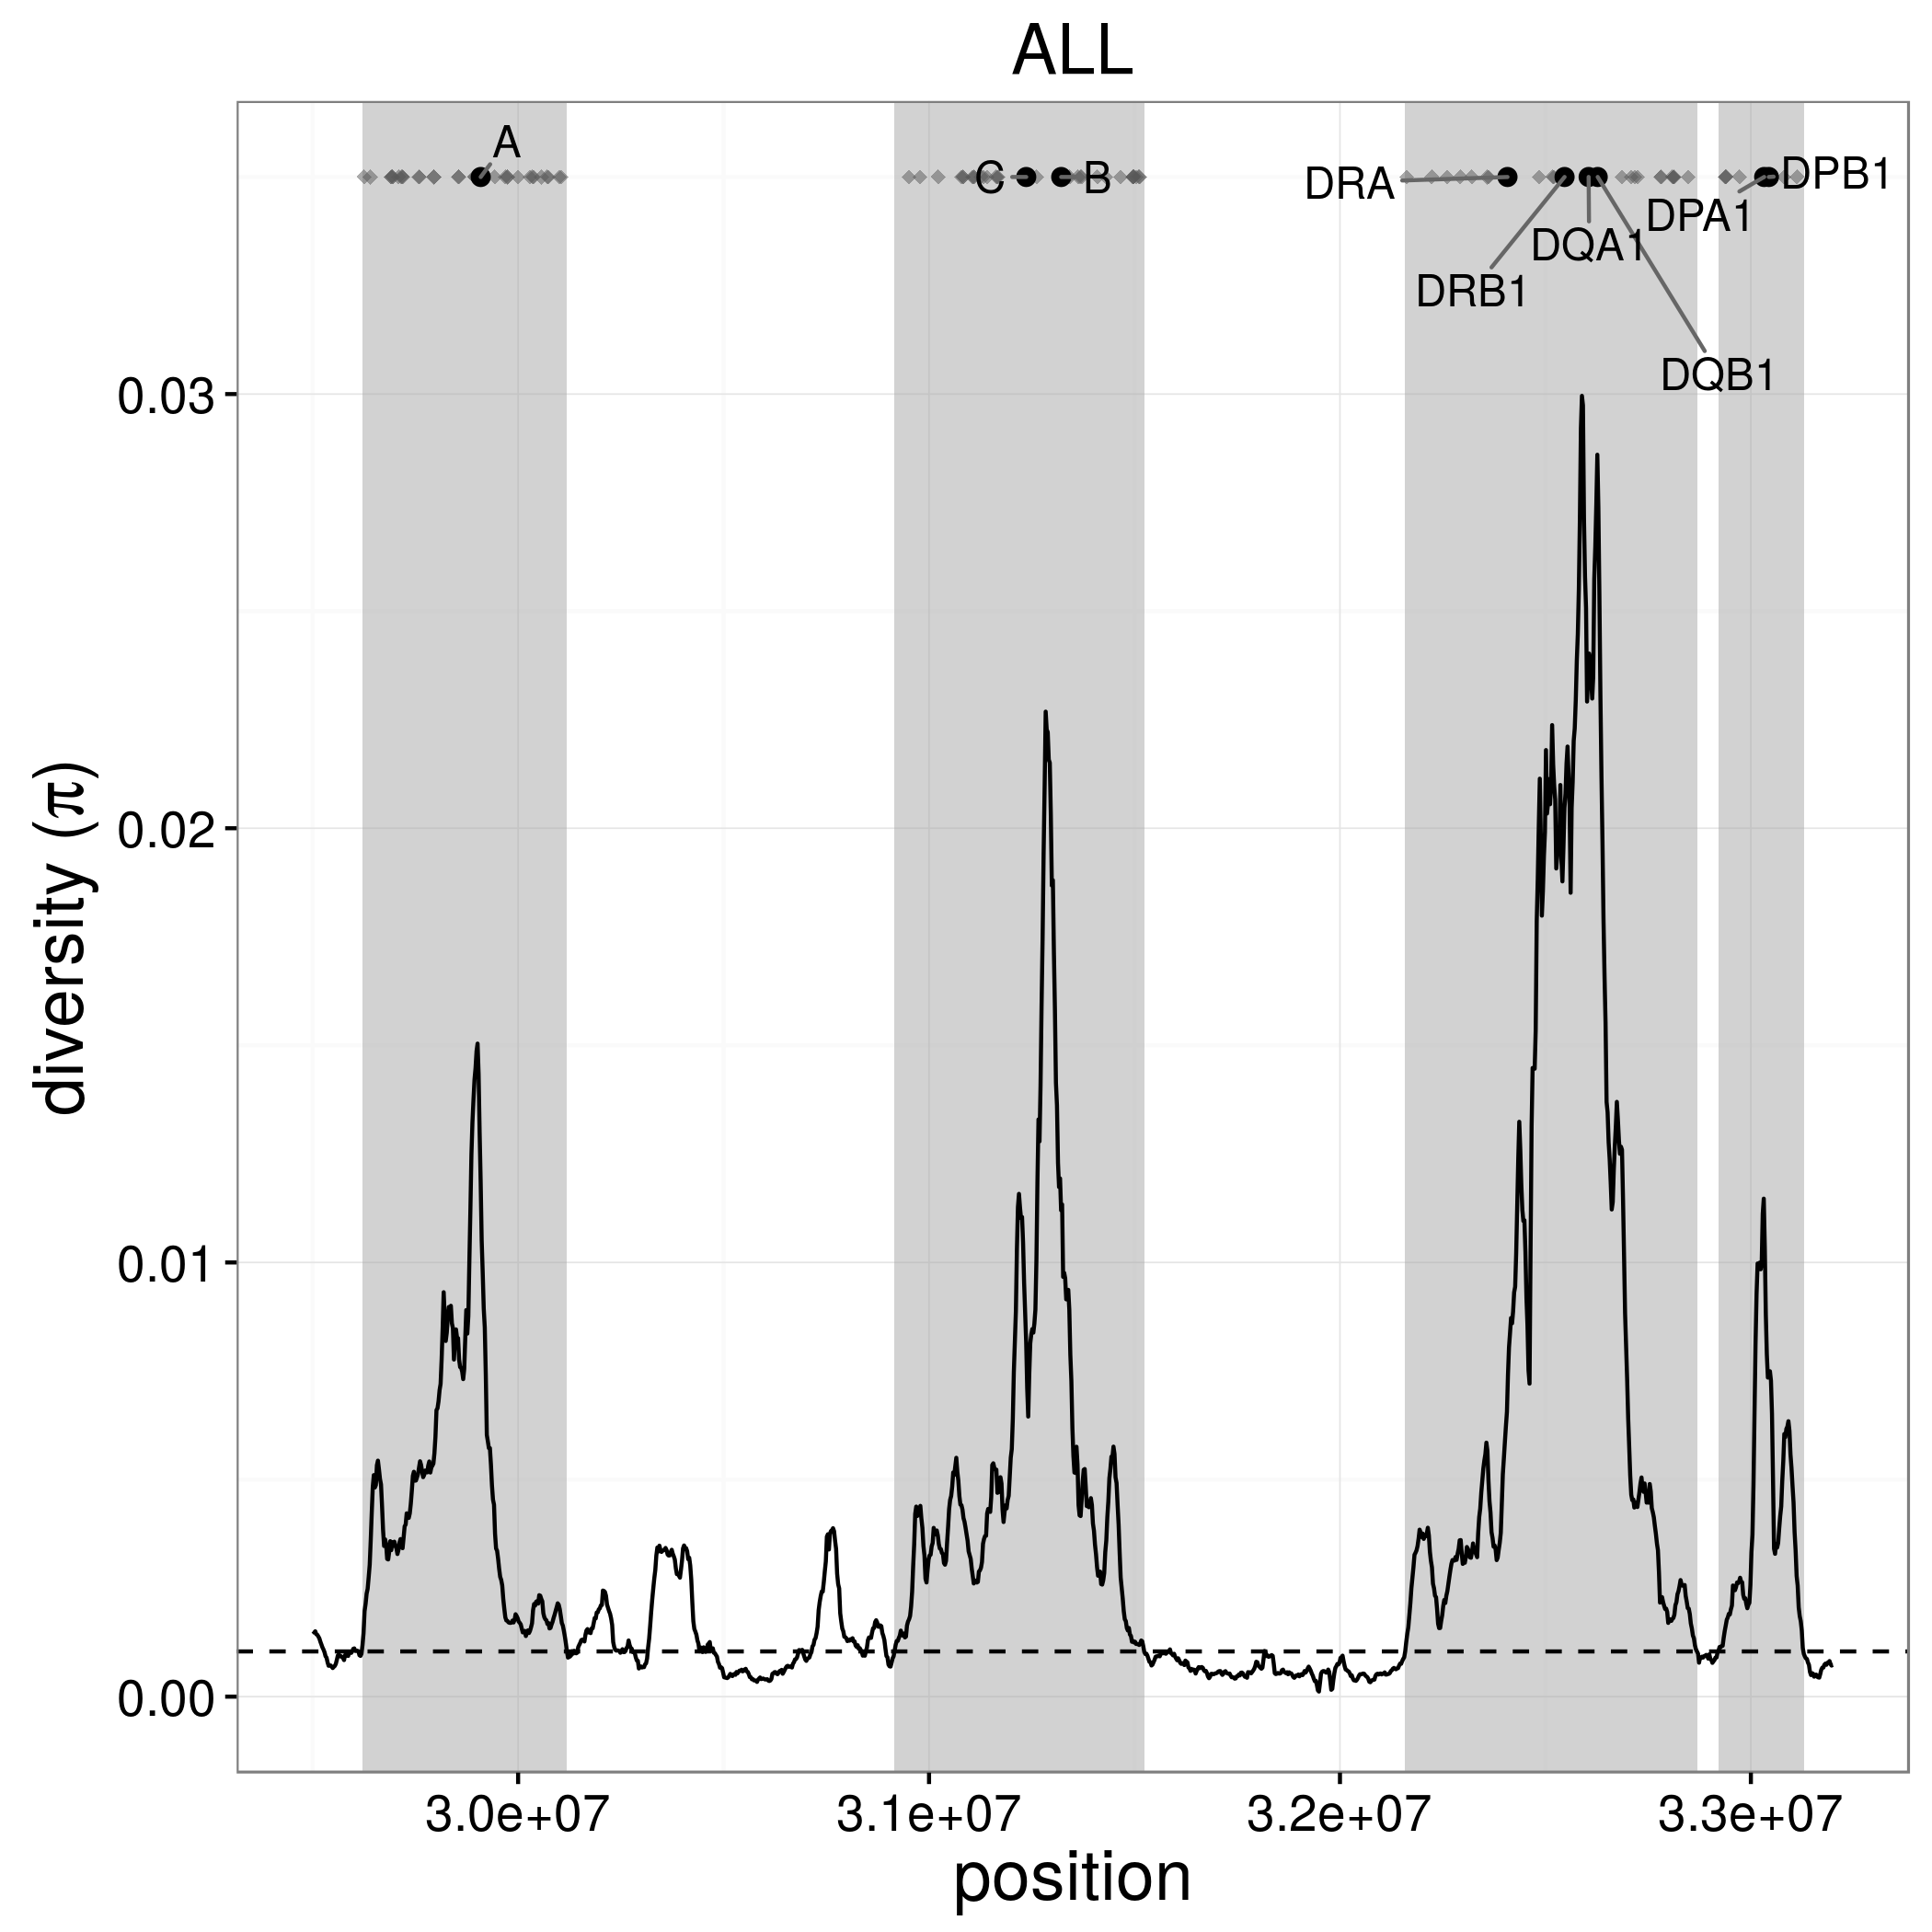
\includegraphics[width=\textwidth]{./Figures/htz_ALL.png}
  \end{minipage}
  \begin{minipage}{0.35\textwidth}
    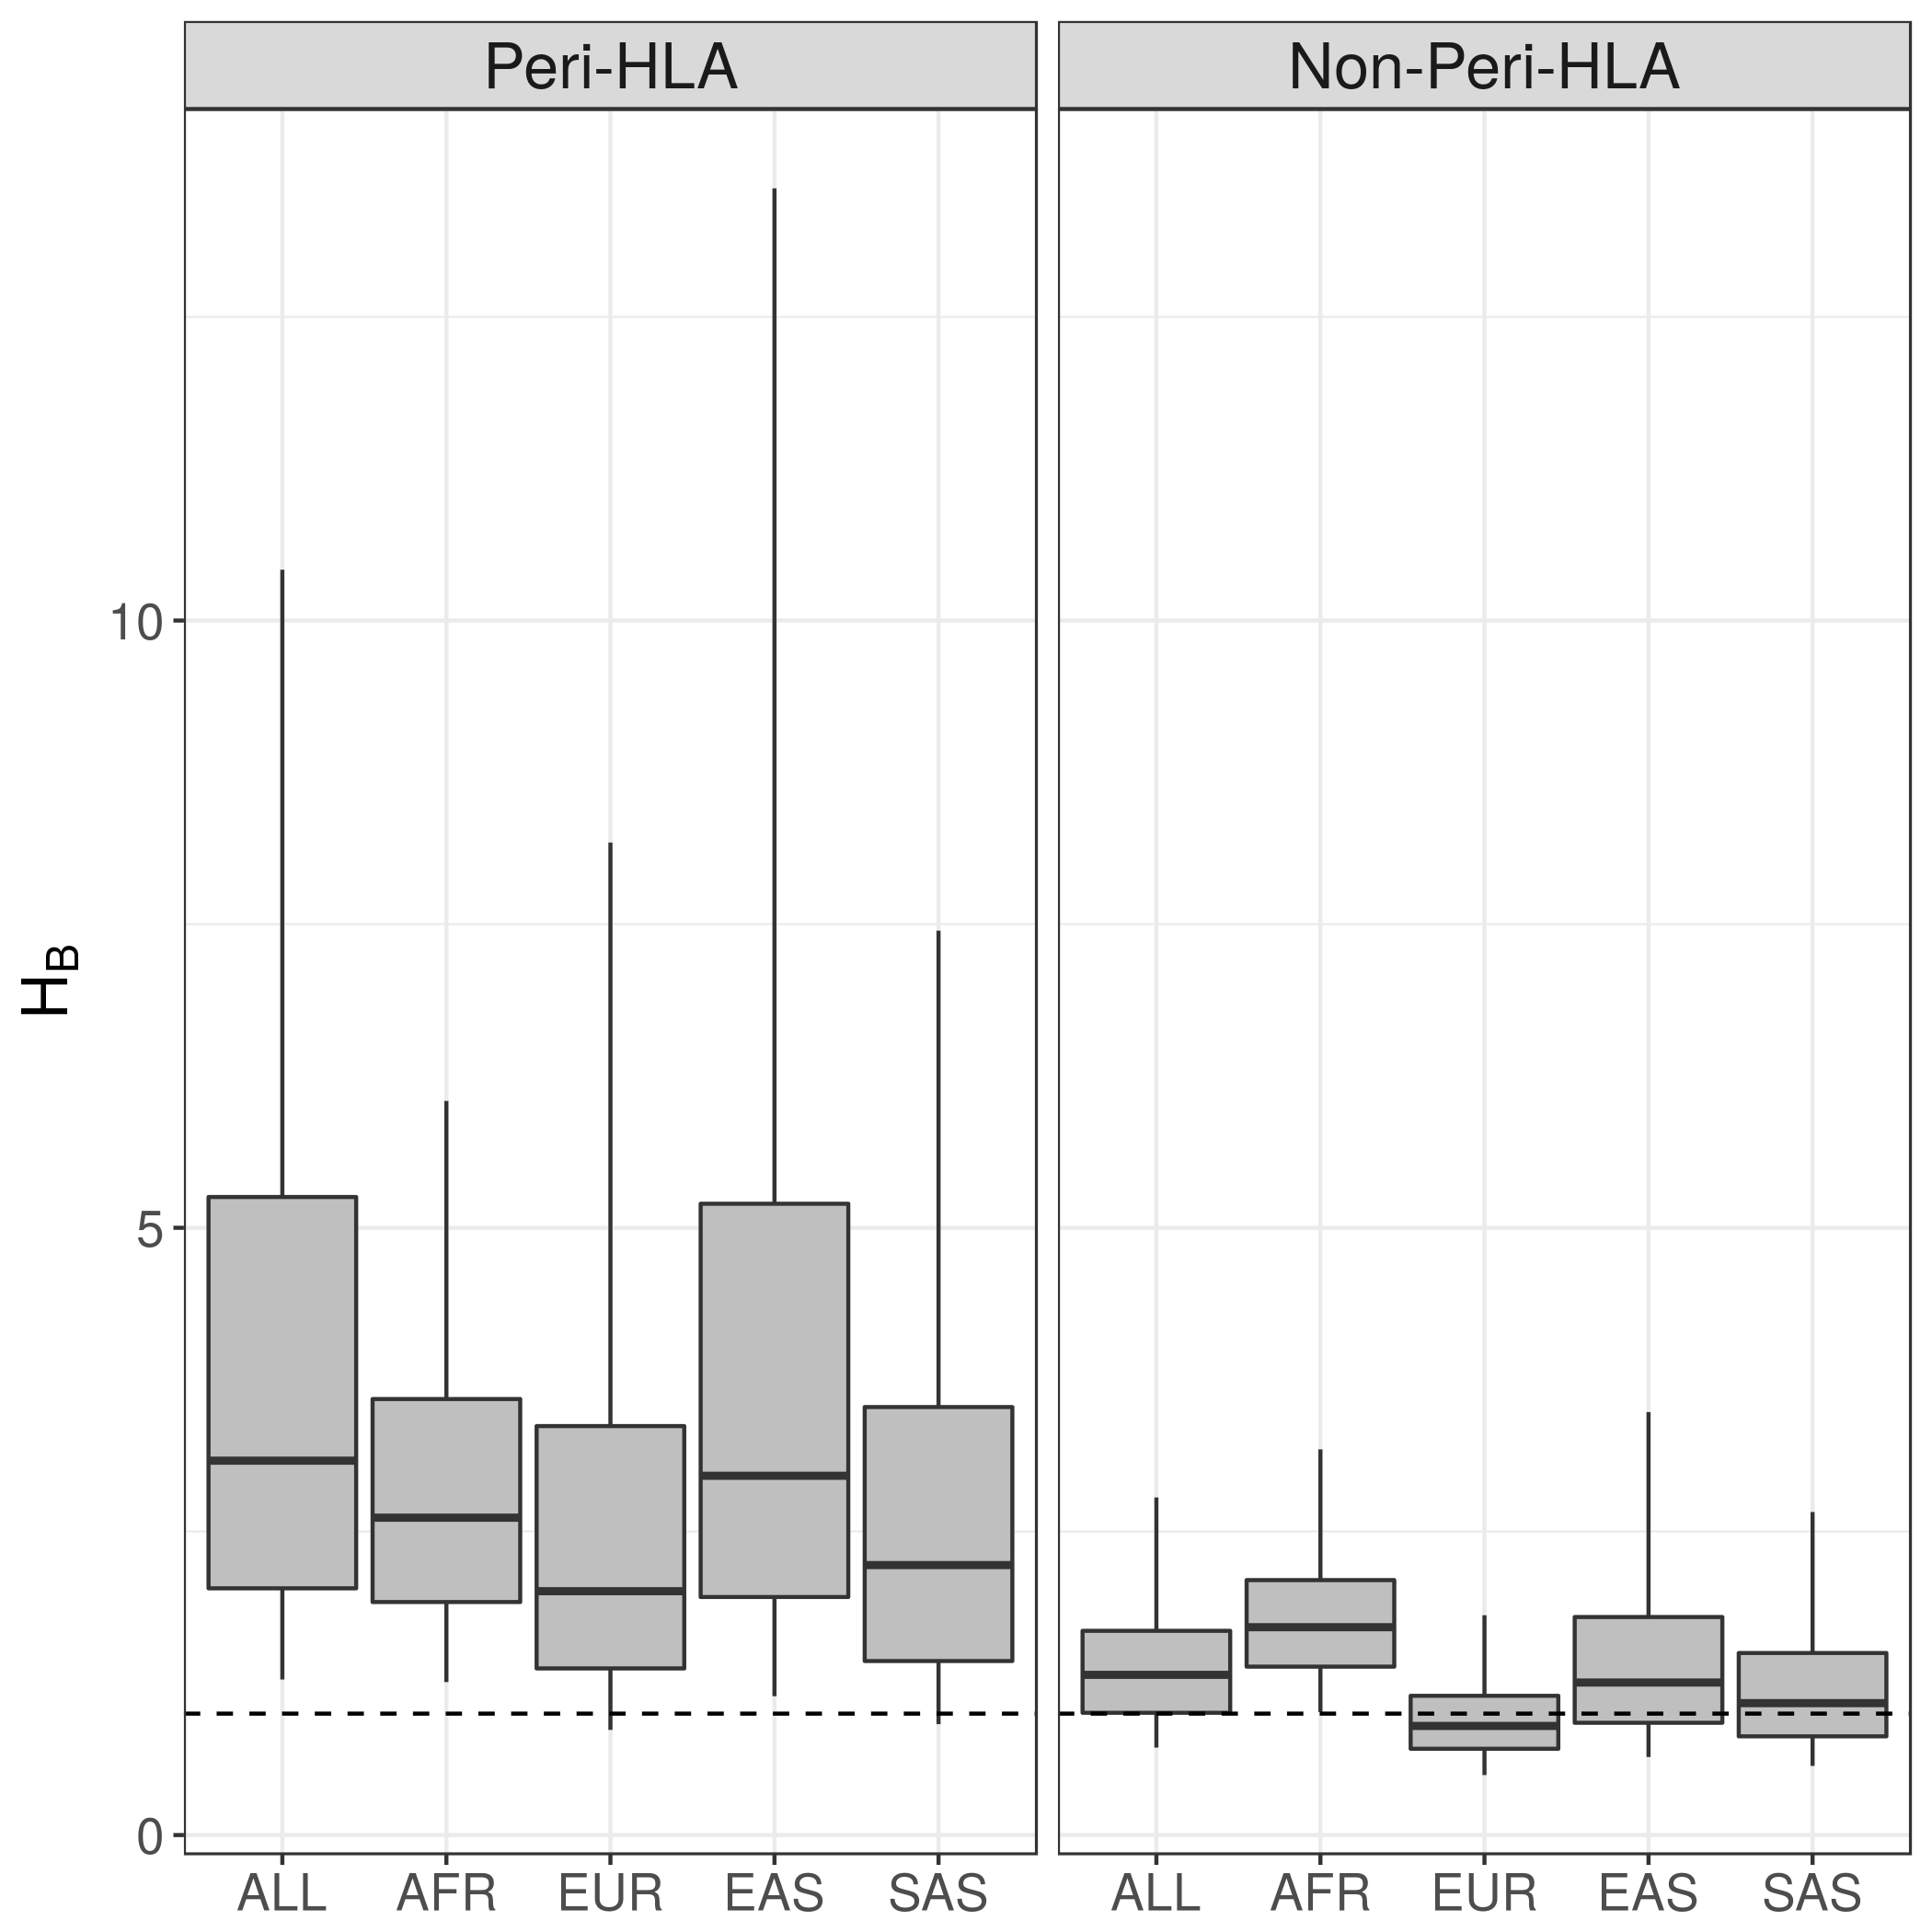
\includegraphics[width=\textwidth]{./Figures/freq_fold_peri.png}
  \end{minipage}
  \begin{minipage}{0.35\textwidth}
    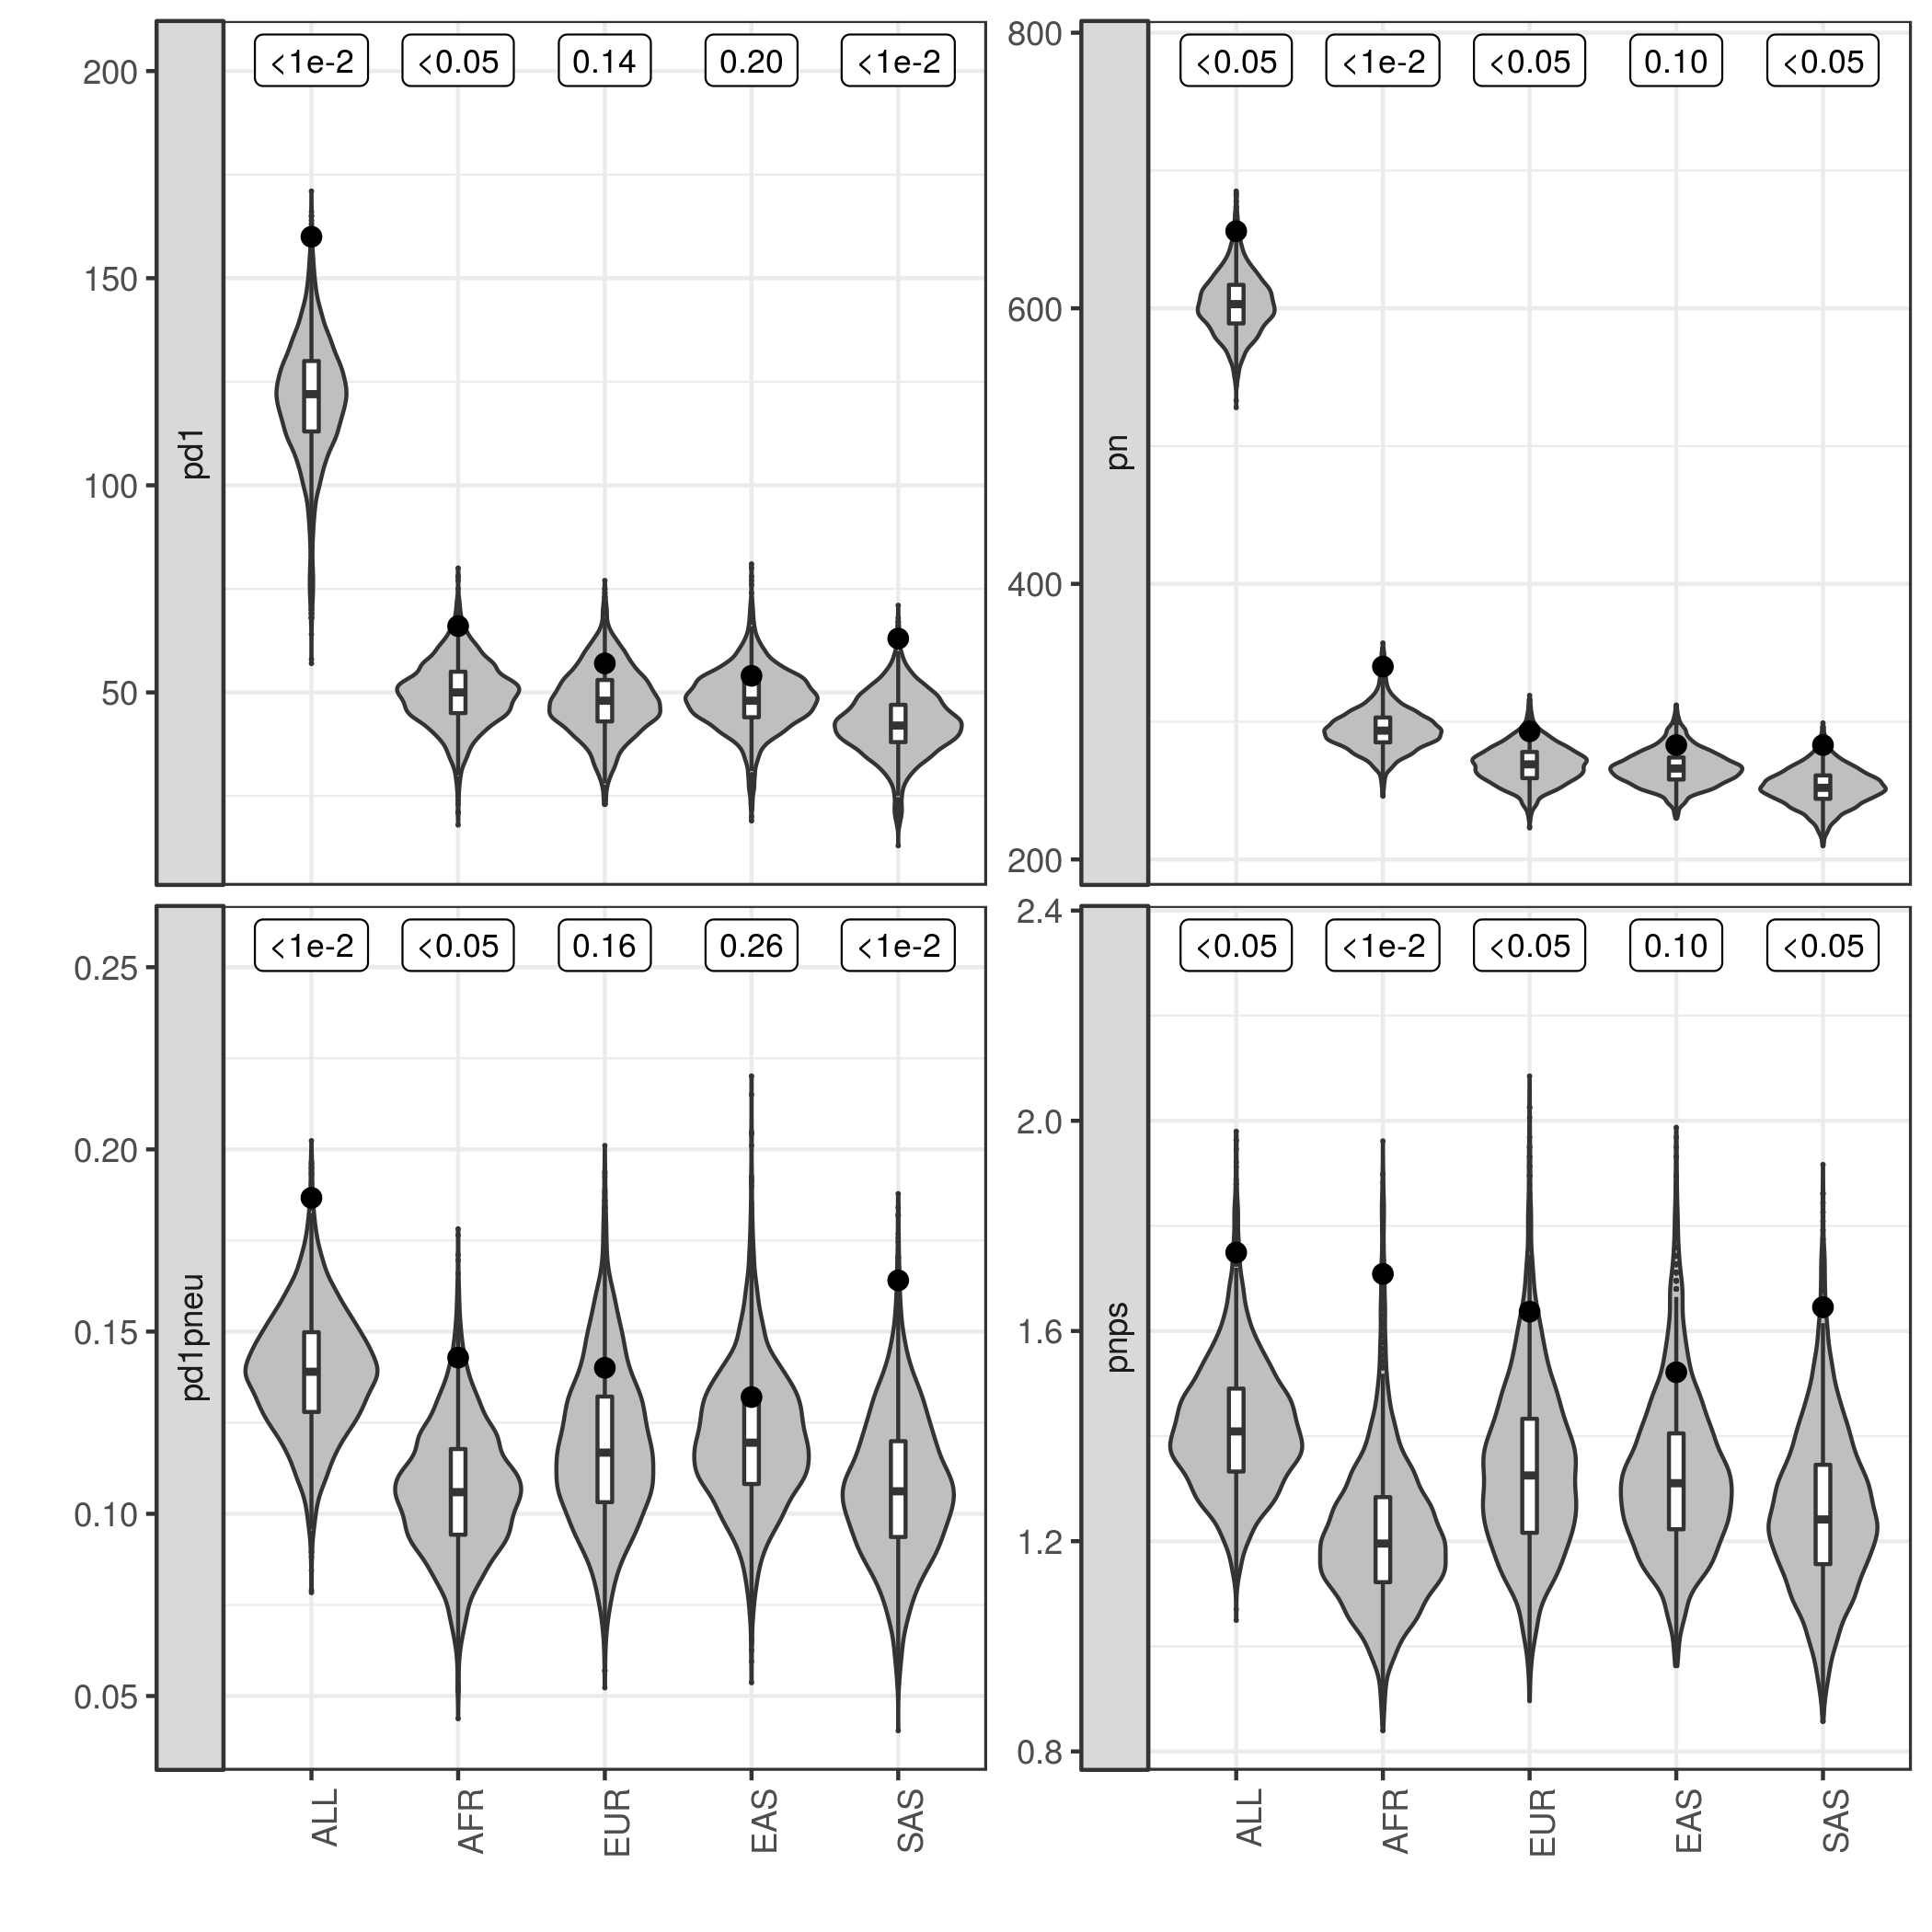
\includegraphics[width=\textwidth]{./Figures/load_Peri.png}
  \end{minipage}
  \begin{minipage}{0.35\textwidth}
    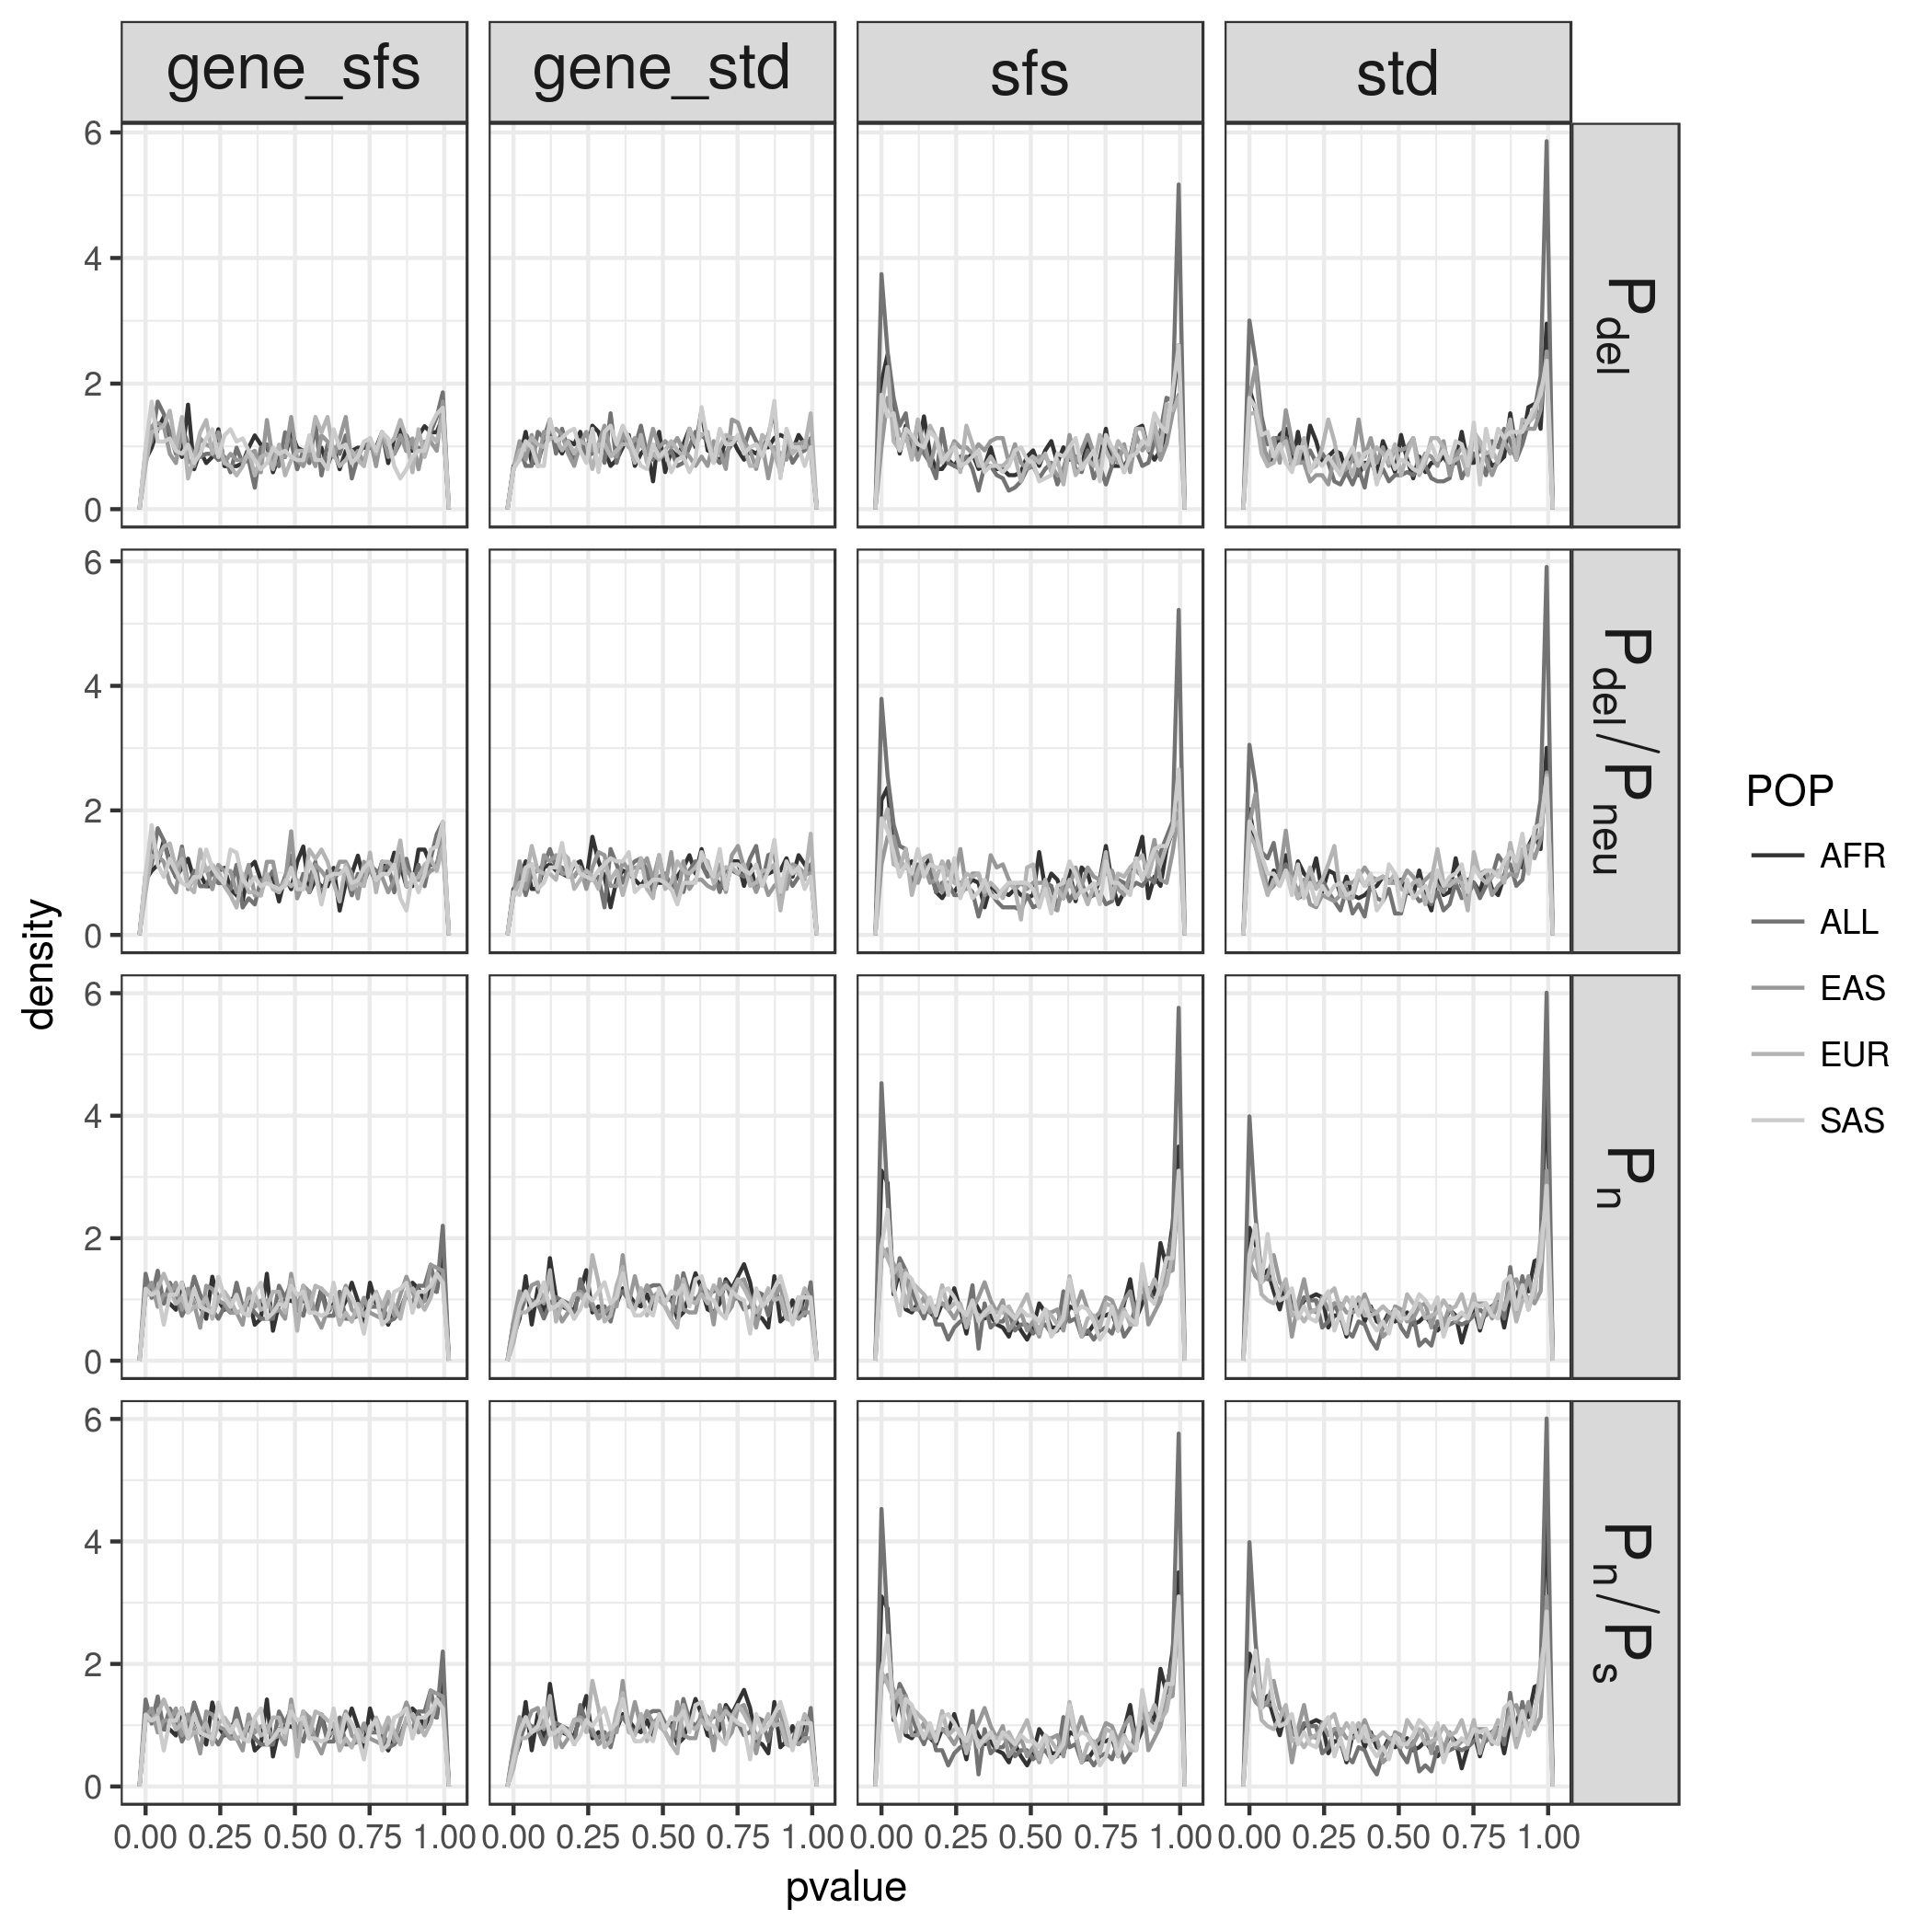
\includegraphics[width=\textwidth]{./Figures/pval_null_hist.png}
  \end{minipage}
  \let\thefootnote\relax\footnote{J. Cesar, \textit{et. al.}, in prep}
\end{frame}

\section{Genetic Load and Efficacy of Selection on admixed populations}

\begin{frame}{Genetic Load}
  \begin{alertblock}{Definition}
    Genetic load is the relative reduction in the population fitness compared
    to the theoretical "perfectly adapted" genotype.
  \end{alertblock}
  \[
    L = \frac{W_{max} - W_{mean}}{W_{max}}
  \]
  Causes:
  \begin{itemize}
    \item \underline{Mutation Load}: Influx of new deleterious mutation
    \item Change in environment
    \item Inbreeding 
    \item ...
  \end{itemize}
\end{frame}

\begin{frame}{Equilibrium Rationale}
\begin{minipage}{0.7\textwidth}
  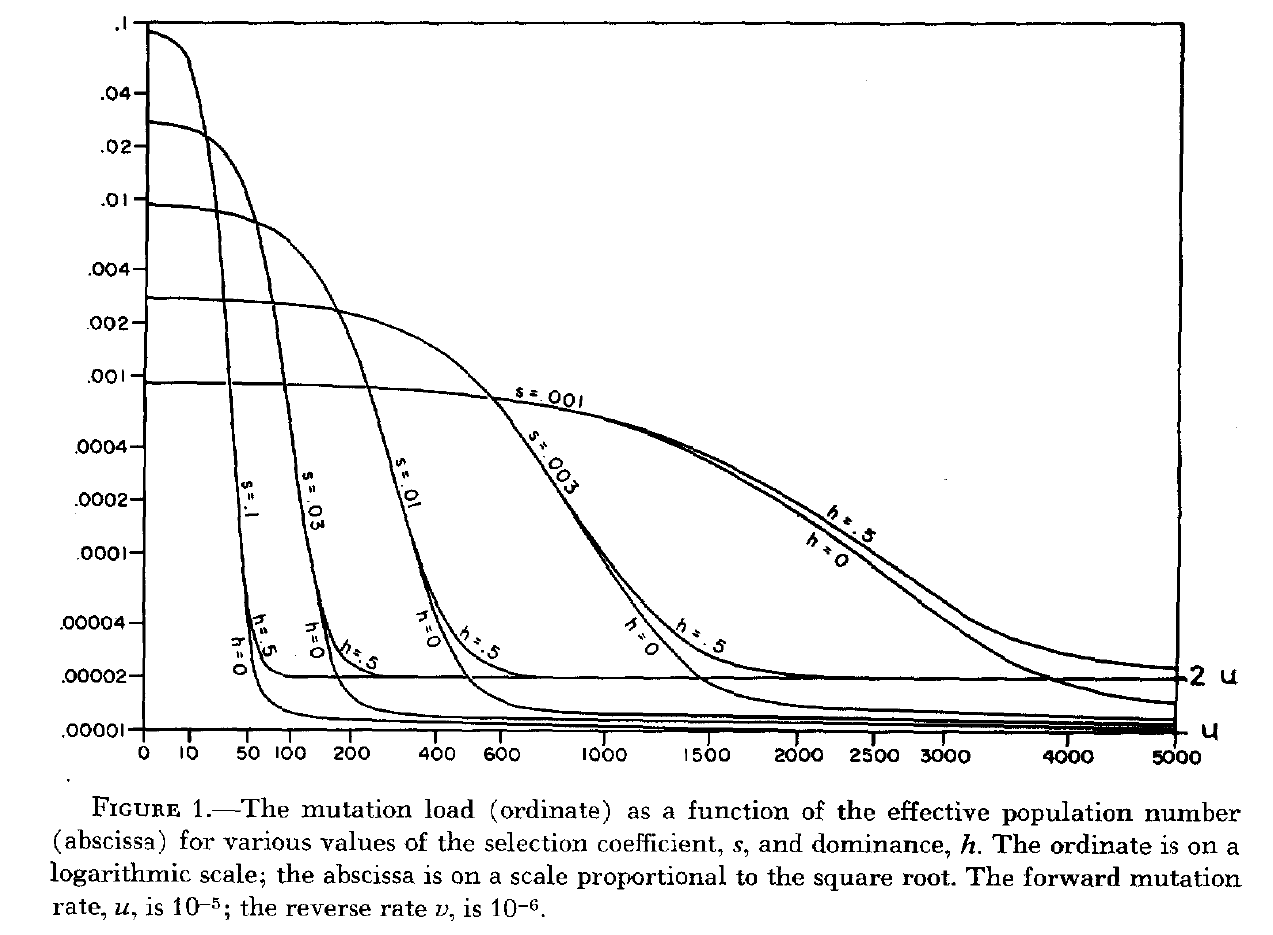
\includegraphics[width=\textwidth]{./Figures/Kimura_1963.png}
\end{minipage}
\end{frame}


\end{document}
